\chapter{Entwurf}\label{desgin}
In diesem Kapitel wird auf verschiedene Aspekte der Entwurfsphase eingegangen.
Zum einen wird dargelegt mit welcher Herangehensweise der Algorithmus umgesetzt wird und zum anderen werden die Entscheidungen über die verwendeten Technologien begründet.

\section{Anforderungen}

Ziel dieser Arbeit ist es, das in \cite*[]{gasperini:hal-03209144} beschriebene Verfahren zu implementieren.
Dabei sind drei Anforderungsbereiche auszumachen, welche in diesem Abschnitt behandelt werden.


\subsection{Korrektheit}

Die trivialste Anforderung ist, den beschriebenen Algorithmus korrekt zu implementieren.
Diese Anforderung ist erfüllt, wenn die Rechenresultate der Implementierung eine Genauigkeit der gleichen Größenordnung wie die MatLab-Implementierung von \cite*[]{gasperini:hal-03209144} erzielen.
Dort werden in Kapitel 6.1 (Tabelle 3) für die Parameter 
\begin{equation}
    A = \begin{pmatrix}
        0 & 0 \\
        2 & 0 \\
        0 & 2 \\
    \end{pmatrix}, b = \begin{pmatrix}
        0 \\ -1 \\ 0
    \end{pmatrix},
    r = \begin{pmatrix}
        0.6 \\ 0 \\0 
    \end{pmatrix},
    \theta = \begin{pmatrix}
        1 \\ 0 \\
    \end{pmatrix}
\end{equation}

die relativen Fehler des implementierten Verfahrens mit der Matlab $integral$ Funktion für verschiedene Wellenzahlen $k$ verglichen.
\begin{table}[ht]
    \centering
    \begin{tabular}{|l|l|}
    \hline
    k & Relativer Fehler \\ 
    \hline \hline
    100  & $1.44 × 10^{-15}$ \\
    500  &  $1.15 × 10^{-14}$ \\
    1000 &  $9.71 × 10^{-5}$ \\
    3000 &  $5.11 × 10^{-7}$ \\
    5000 & $1.31 × 10^{-8}$ \\  \hline
    \end{tabular}    
    \caption{Genauigkeit der Implementierung von \cite*[]{gasperini:hal-03209144}}
\end{table} 
Das Kriterium der Korrektheit wird als erfüllt angesehen, wenn die Implementierung höchstens Fehler der gleichen Größenordnung liefert.


\subsection{Bedienbarkeit}

Die Anforderung der Bedienbarkeit wird im Rahmen dieser Arbeit wie folgt definiert:

\begin{enumerate}
    \item Es wird eine C++-Bibliothek bereitgstellt, welche mithilfe des Build-System \textit{CMake} eingebunden werden kann. 
    \item Es wird eine oder mehrere Matlab-Mex Funktionen ausgeliefert, welche den Algorithmus in Matlab benutzbar machen. 
    \item Es wird ein Python-Modul bereitgesellt, mit dem die 1D und 2D Algorithmen genutzt werden können.
\end{enumerate}

Dabei ist es nicht das Ziel, die beschriebenen Pakete offiziel auszuliefern. Das eigenhändige Compilieren der Bilbiothek und ggf. der Module ist erforderlich.

\subsection{Geschwindigkeit}\label{Performance}


Der implementierte Algorithmus darf nicht langsamer als die bereitgestellte Matlab-Implementierung sein.
Zu diesesm Zweck werden einige Auswertungen mit randomisierten Daten mithilfe von MatLab ausgeführt und direkt mit der vorhandenen MatLab-Implementierung verglichen.



\section{Architektur}

Diese Arbeit wird mit der Programmiersprache C++ umgesetzt.
Die Anwendung wird in drei Module aufgeteilt. 
Die Hauptbibliothek \texttt{steepest\_descent}, in welcher der eigentliche Algorithmus implementiert wird.
Diese API-Endpunkte dienen den Python- und Matlab-Wrappern die nötigen Anknüpfpunkte. 
\\
Das Python-Modul \texttt{stedepy} welches die in der Hauptbibliothek API-Endpunkte bereitstellt, sowie eine Möglichkeit, die benötigten Gauss-Laguerre-Knoten vorab zu berechnen.
Das Matlab-Modul, welches sich aus mehreren Mex-Funktionen zusammensetzt, welche die Funkionen der API bereitstellen.
\\
\subsection{Klassendiagramm}

In Abbildung \ref{uml} wird ein vereinfachter Überblick über die implementierten Klassen und ihr Zusammenwirken gegeben.
Die Klassen \texttt{integral\_1d} und \texttt{integral\_2d} sind dabei die Schnittstellen für das Python und das Matlab Modul.
Die dargestellten Klassen sind verkürzt und die Funktionsparameter wurden ausgelassen, um die Lesbarkeit zu erhalten.

\begin{figure}
    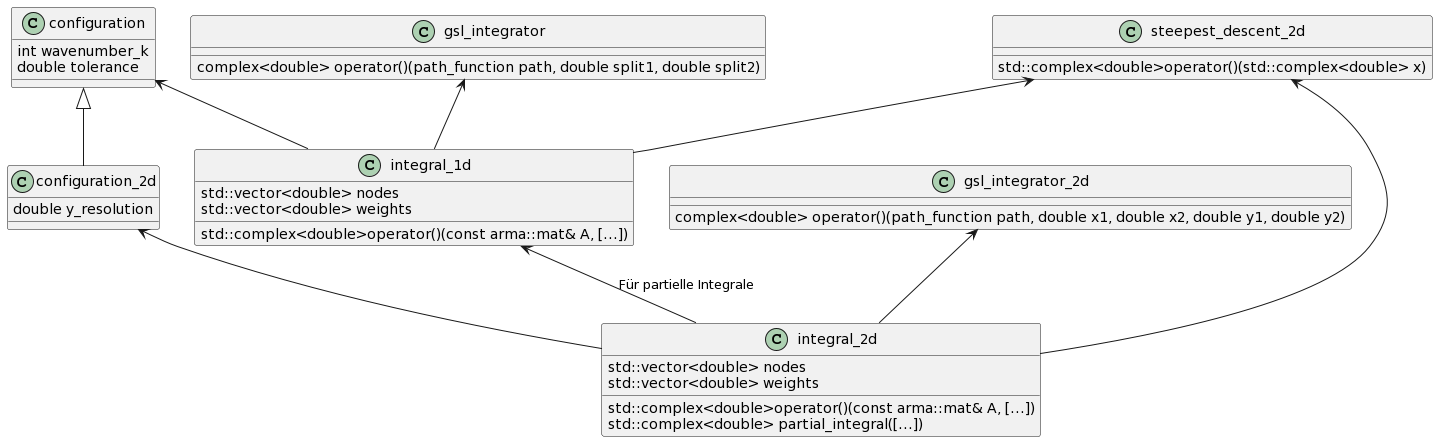
\includegraphics[width=\textwidth]{images/uml.png}
    \caption{Vereinfachtes UML-Diagramm der Implementierung}\label{uml}
\end{figure}

\pagebreak

\subsection{Parameter der Integration}

Die einzelnen API-Aufrufe teilen nur wenige gemeinsame Daten:
\begin{itemize}
    \item Die Wellenzahl $k$,
    \item den Beobachtungspunkt $r$,
    \item die Anzahl an Knoten für das Gauss-Laguerre-Verfahren,
    \item sowie die gewünschte Auflösung im zweidimensionalen Fall
\end{itemize}
Diese werden, abgesehen von dem Beobachtungspunkt $r$, in einer Konfigurationsklasse (siehe Abbildung \ref{configuration}) zusammengefasst.

\begin{figure}
    \lstinputlisting[language=C++,style=cpp]{configuration2d.cpp}
    \caption{Die Konfigurationen}\label{configuration}
\end{figure}


Die Parameter einer Integration eines Dreiecks teilen sich wie folgt auf:

\begin{itemize}
    \item Das Dreieck als parametrisiertes Einheitsdreieck, bestehend aus einer $2\times 3$-Matrix $A$ und einem Verschiebungsvektor $b$,
    \item der Beobachtungspunkt $r$,
    \item ein Richtungsvektor $\theta$
\end{itemize}

Zusätzlich wird noch der Beobachtungspunkt als Parameter mitgereicht, dies ermöglicht eine vollständige Kompabilität mit der Matlab-Implementierung.

\subsection{Functor-Objekte}\label{sec_functor}

Die Hauptkomponenten zur Integrationen werden als sogenannte \textit{Functor}-Objekte (Funktor) implementiert.
Diese Datenstruktur zeichnet sich dadurch aus, dass sie den C++-Funktionsaufrufsoperator bereitstellen und wie einfache C++-Funktionen aufgerufen werden können.
Da Funktoren durch Klassen bzw. \textit{structs} definiert werden, kann in ihnen ein Zustand gespeichert werden.
In Abbildung \ref{2d_integral_functor} ist die Header-Definition des Funktor für das Berechnen des zweidimensionalen Falls gezeigt.
In den Konstruktoren werden Parameter übergeben, welche für mehr als eine Integration invariant sind. In der Implementierung des Funktionsaufrufsoperators werden die im vorherigen Abschnitt definierten Parameter erwartet.

\begin{center}
    \lstinputlisting[language=C++,style=cpp]{2d_integral.hpp}
    \captionof{figure}{Funktordefinition der zweidimensionalen Integration}
    \label{2d_integral_functor}
\end{center}